%	This is written by Zhiyang Ong as a template for writing reports.

%	The MIT License (MIT)

%	Copyright (c) <2014> <Zhiyang Ong>

%	Permission is hereby granted, free of charge, to any person obtaining a copy of this software and associated documentation files (the "Software"), to deal in the Software without restriction, including without limitation the rights to use, copy, modify, merge, publish, distribute, sublicense, and/or sell copies of the Software, and to permit persons to whom the Software is furnished to do so, subject to the following conditions:

%	The above copyright notice and this permission notice shall be included in all copies or substantial portions of the Software.

%	THE SOFTWARE IS PROVIDED "AS IS", WITHOUT WARRANTY OF ANY KIND, EXPRESS OR IMPLIED, INCLUDING BUT NOT LIMITED TO THE WARRANTIES OF MERCHANTABILITY, FITNESS FOR A PARTICULAR PURPOSE AND NONINFRINGEMENT. IN NO EVENT SHALL THE AUTHORS OR COPYRIGHT HOLDERS BE LIABLE FOR ANY CLAIM, DAMAGES OR OTHER LIABILITY, WHETHER IN AN ACTION OF CONTRACT, TORT OR OTHERWISE, ARISING FROM, OUT OF OR IN CONNECTION WITH THE SOFTWARE OR THE USE OR OTHER DEALINGS IN THE SOFTWARE.

%	Email address: echo "cukj -wb- 23wU4X5M589 TROJANS cqkH wiuz2y 0f Mw Stanford" | awk '{ sub("23wU4X5M589","F.d_c_b. ") sub("Stanford","d0mA1n"); print $5, $2, $8; for (i=1; i<=1; i++) print "6\b"; print $9, $7, $6 }' | sed y/kqcbuHwM62z/gnotrzadqmC/ | tr 'q' ' ' | tr -d [:cntrl:] | tr -d 'ir' | tr y "\n"

%%%%%%%%%%%%%%%%%%%%%%%%%%%%%%%%%%%%%%%%%%%%%%


%%%%%%%%%%%%%%%%%%%%%%%%%%%%%%%%%%%%%%%%%%%
\section{Multi-Cycle Processor Design}
\label{sec:MultiCycleProcessorDesign}


%	Figure 5.39 and 5.40 from \cite{Patterson2005}
To improve the performance of the single-cycle {\it MIPS} processor (see \S\ref{sec:SingleCycleProcessorDesign}), a better semiconductor manufacturing process technology can be used to manufacture implementations of the microarchitecture as a VLSI system. Alternatively, the microarchitecture can be modified to significantly improve the performance of the processor. For each instruction in the {\it MIPS} ISA, decompose the instruction into steps based on the functional units required to complete executing that instruction. That is, if an instruction needs five components, it shall be decomposed/partitioned into five steps. Each step of the decomposed instruction shall take one clock cycle. In general, the datapath in Subsection \ref{ssec:DatapathDesignforSingleCycleProcessors} (see Figure \ref{fig:mipsdatapath}) can be decomposed into the following five stages \cite{Patterson2005}: \vspace{-0.3cm}
\begin{enumerate} \itemsep -4pt
\item Instruction fetch (IF). Instructions are fetched from memory and the program counter (PC) is updated.
\item Instruction decode (ID). Instructions are decoded and register(s) are read from the register file {\tt regfile}.
\item Execution (EX). Arithmetic/logical operations are performed by the arithmetic-logical unit (ALU).
\item Memory access (MEM). Read data from or write data to the memory device or memory system (including caches).
\item Write-back (WB). Complete memory read operations (i.e., load operations).
\end{enumerate}

Each of the stages listed above can be a step for a decomposed instruction. Since different instructions require different number of stages, the CPI for instructions in the {\it MIPS} ISA would vary for microarchitectures that allow instructions to complete in a range of clock cycles. These microarchitectures are known as multi-cycle processors. A multi-cycle processor allows a functional unit to be used multiple times per clock cycle. This reduces the amount of required hardware resources/components and encourages microarchitects (or processor architects) to share hardware resources between different steps of an instruction \cite{Patterson2005}. \\

The rest of this section is organized as follows. In Subsection \ref{ssec:DatapathDesignforMultiCycleProcessors}, I discuss the datapath design for the multi-cycle {\it MIPS} processor. Following this, in Subection \ref{ssec:ControlPathDesignforMultiCycleProcessors}, I describe the control path of the multi-cycle {\it MIPS} processor, including a brief discussion of how to implement the finite state machine representation of the control unit (in the control path) as a sequential circuit (see \S\ref{sssec:FiniteStateControl}). Next, I compare the advantages and disadvantages of the multi-cycle {\it MIPS} processor with the single-cycle {\it MIPS} processor (see \S\ref{sec:SingleCycleProcessorDesign}) in Subsection \ref{ssec:AdvantagesandDisadvantagesofMultiCycleProcessorDesign}. Lastly, in Subsection \ref{ssec:Microprogramming}, I discuss how microprogramming can be used to reduce the hardware complexity of a microarchitecture's control path, and reduce the amount of effort needed to design that microarchitecture as a VLSI system.



%%%%%%%%%%%%%%%%%%%%%%%%%%%%%%%%%%%%%%%%%%%
\subsection{Datapath Design for Multi-Cycle Processor}
\label{ssec:DatapathDesignforMultiCycleProcessors}

\begin{figure}[h]
\centering 
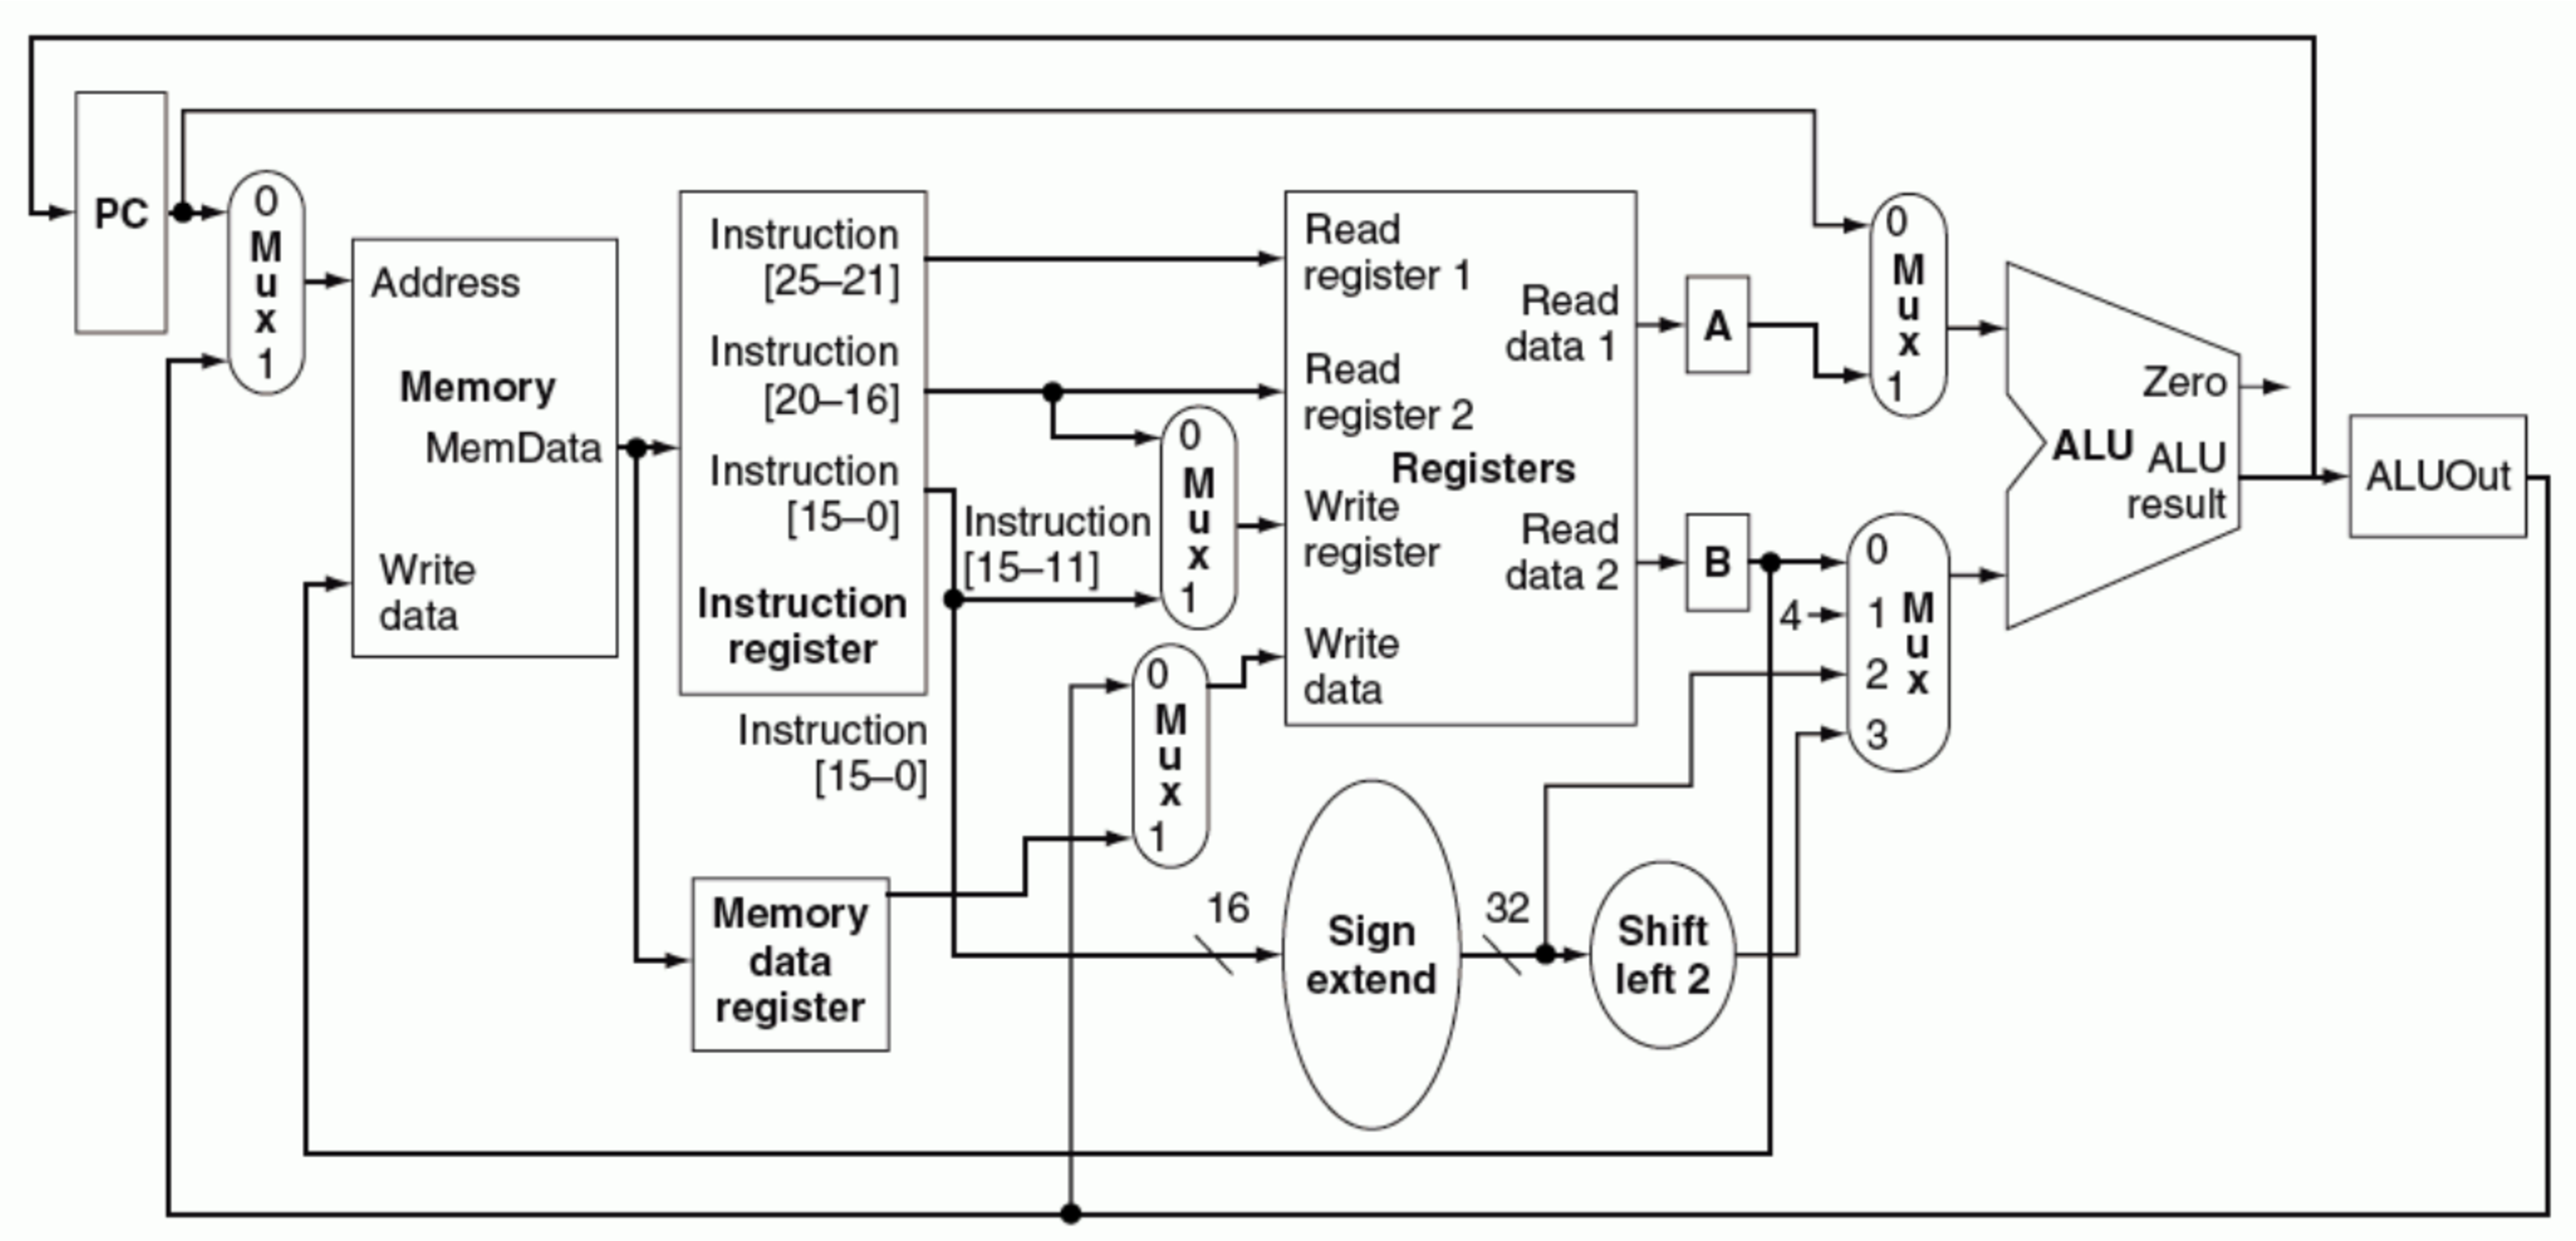
\includegraphics[width=6in]{./pics/multi-cycle-processor-data-path2}
\caption{Datapath of a multi-cycle {\it MIPS} processor \cite{Patterson2005}.}
\label{fig:multicycleprocessordatapath2}
\end{figure}
%	Figure 5.39, \cite{Patterson2005}, pp. 344


Figure \ref{fig:multicycleprocessordatapath2} shows the datapath of a multi-cycle {\it MIPS} processor \cite{Patterson2005}. The datapath design is obtained by partitioning the datapath of the single-cycle {\it MIPS} processor into hardware components needed for decomposed steps of instructions. As aforementioned, datapath components (or hardware resources in the datapath) of the single-cycle {\it MIPS} processor (see Figure \ref{fig:singlecycleprocessor}) are shared to reduce the number of components in the datapath. For example, the data and instruction memory devices are combined into a memory device for data and instructions. In addition, only one ALU is needed in the datapath, since it can be reused in different clock cycles during the execution of an instruction \cite{Patterson2005}. \\

For a given instruction, it can use data for multiple clock cycles, since an instruction would require more than two clock cycles to load and complete execution. Therefore, state elements are used to provide this data for multiple clock cycles. State elements are visible to software developers and include the following: PC counter, register file, memory device/system, and registers (for temporary storage of data that will be used in later cycles of a given instruction). The following temporary registers are added to the microarchitecture of the multi-cycle {\it MIPS} processor \cite{Patterson2005}: \vspace{-0.3cm}
\begin{enumerate} \itemsep -4pt
\item Instruction register (IR). IR is used to save the output of an instruction read operation for use in the same clock cycle.
\item Memory data register (MDR). MDR is used to save the output of an data read operation for use in the same clock cycle.
\item Registers {\tt A} and {\tt B}. They are used to hold the values of register operands of an instruction and serve as a buffer between the register file and the ALU.
\item Register {\tt ALUOut}. It holds the output of the ALU.
\end{enumerate}

Therefore, for the multi-cycle {\it MIPS} processor to function correctly, the clock cycle has to be determined by the longest latency of the aforementioned five stages. In turn, this determines the performance of the multi-cycle {\it MIPS} processor.


%%%%%%%%%%%%%%%%%%%%%%%%%%%%%%%%%%%%%%%%%%%
\subsection{Control Path Design for Multi-Cycle Processor}
\label{ssec:ControlPathDesignforMultiCycleProcessors}

\begin{figure}[h]
\centering 
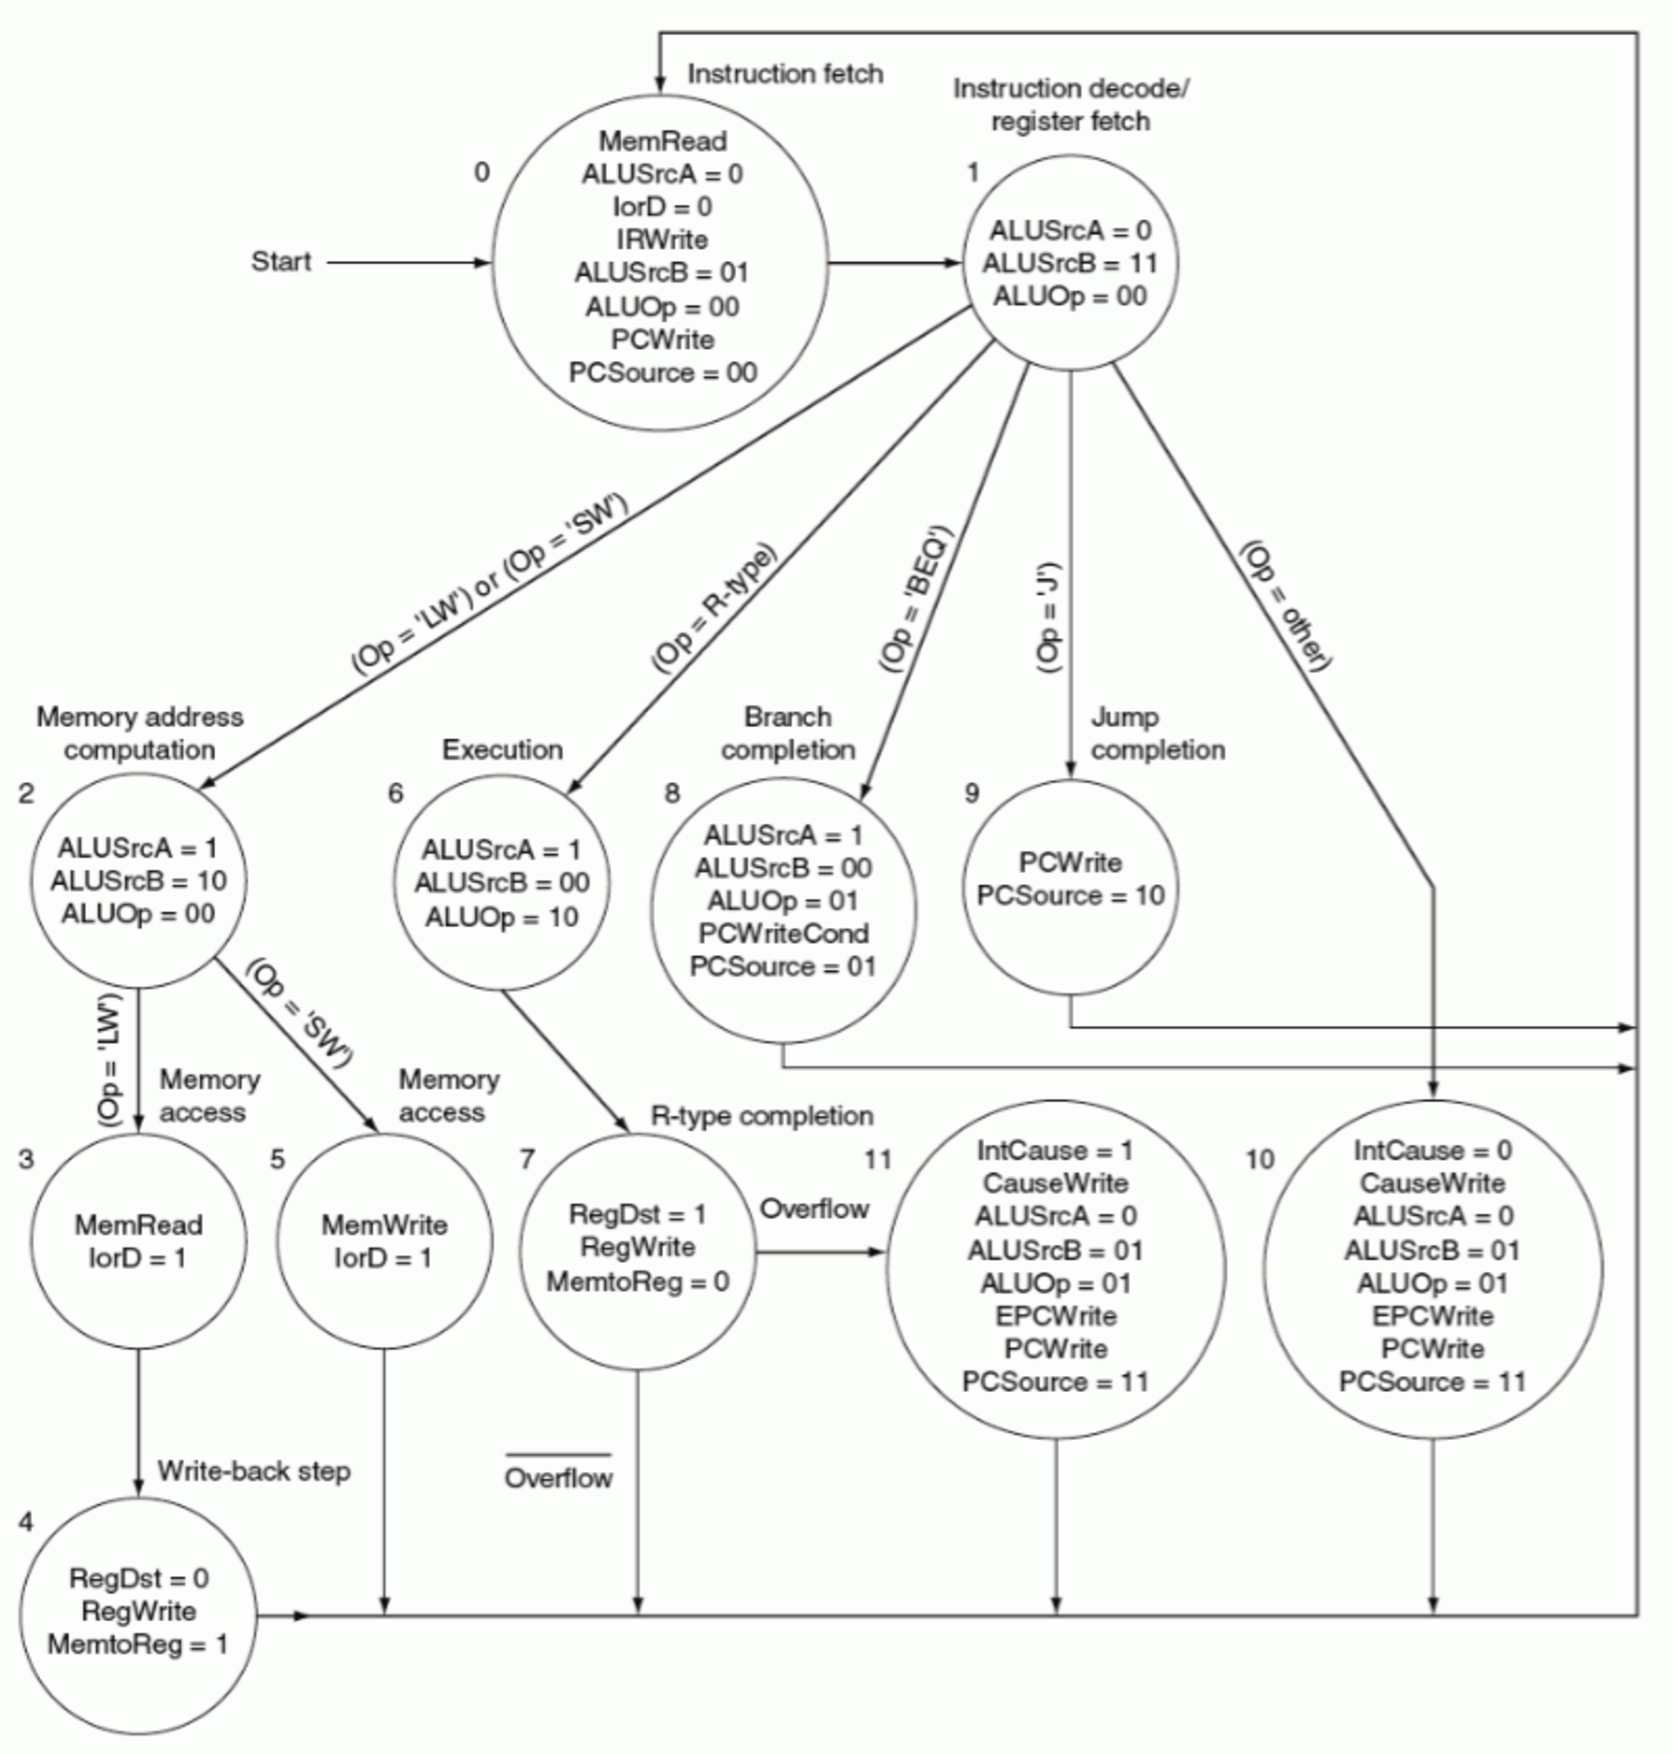
\includegraphics[width=6in]{./pics/multi-cycle-processor-fsm-ctrl-logic}
\caption{Finite state machine representation of the control unit for a multi-cycle {\it MIPS} processor \cite{Patterson2005,Patterson2005a}.}
\label{fig:multicycleprocessorfsmctrllogic}
\end{figure}
%	Figure 5.40, \cite{Patterson2005}, pp. 345

The control unit for a multi-cycle {\it MIPS} processor has multiple sequential states. Therefore, this control unit needs to be implemented as a sequential logic circuit. The sequential behavior of a sequential logic/digital circuit can be represented as a finite state machine (FSM) \cite{Patterson2005a}. Subsection \ref{sssec:FiniteStateControl} provides a description of transforming a FSM representation of the control unit into a sequential digital circuit. Alternatively, microprograms can be used to implement the control path of the processor and simplify the microarchitecture design of the multi-cycle processor (see \S\ref{ssec:Microprogramming}) \cite{Patterson2005}. \\


\begin{figure}[h]
\centering 
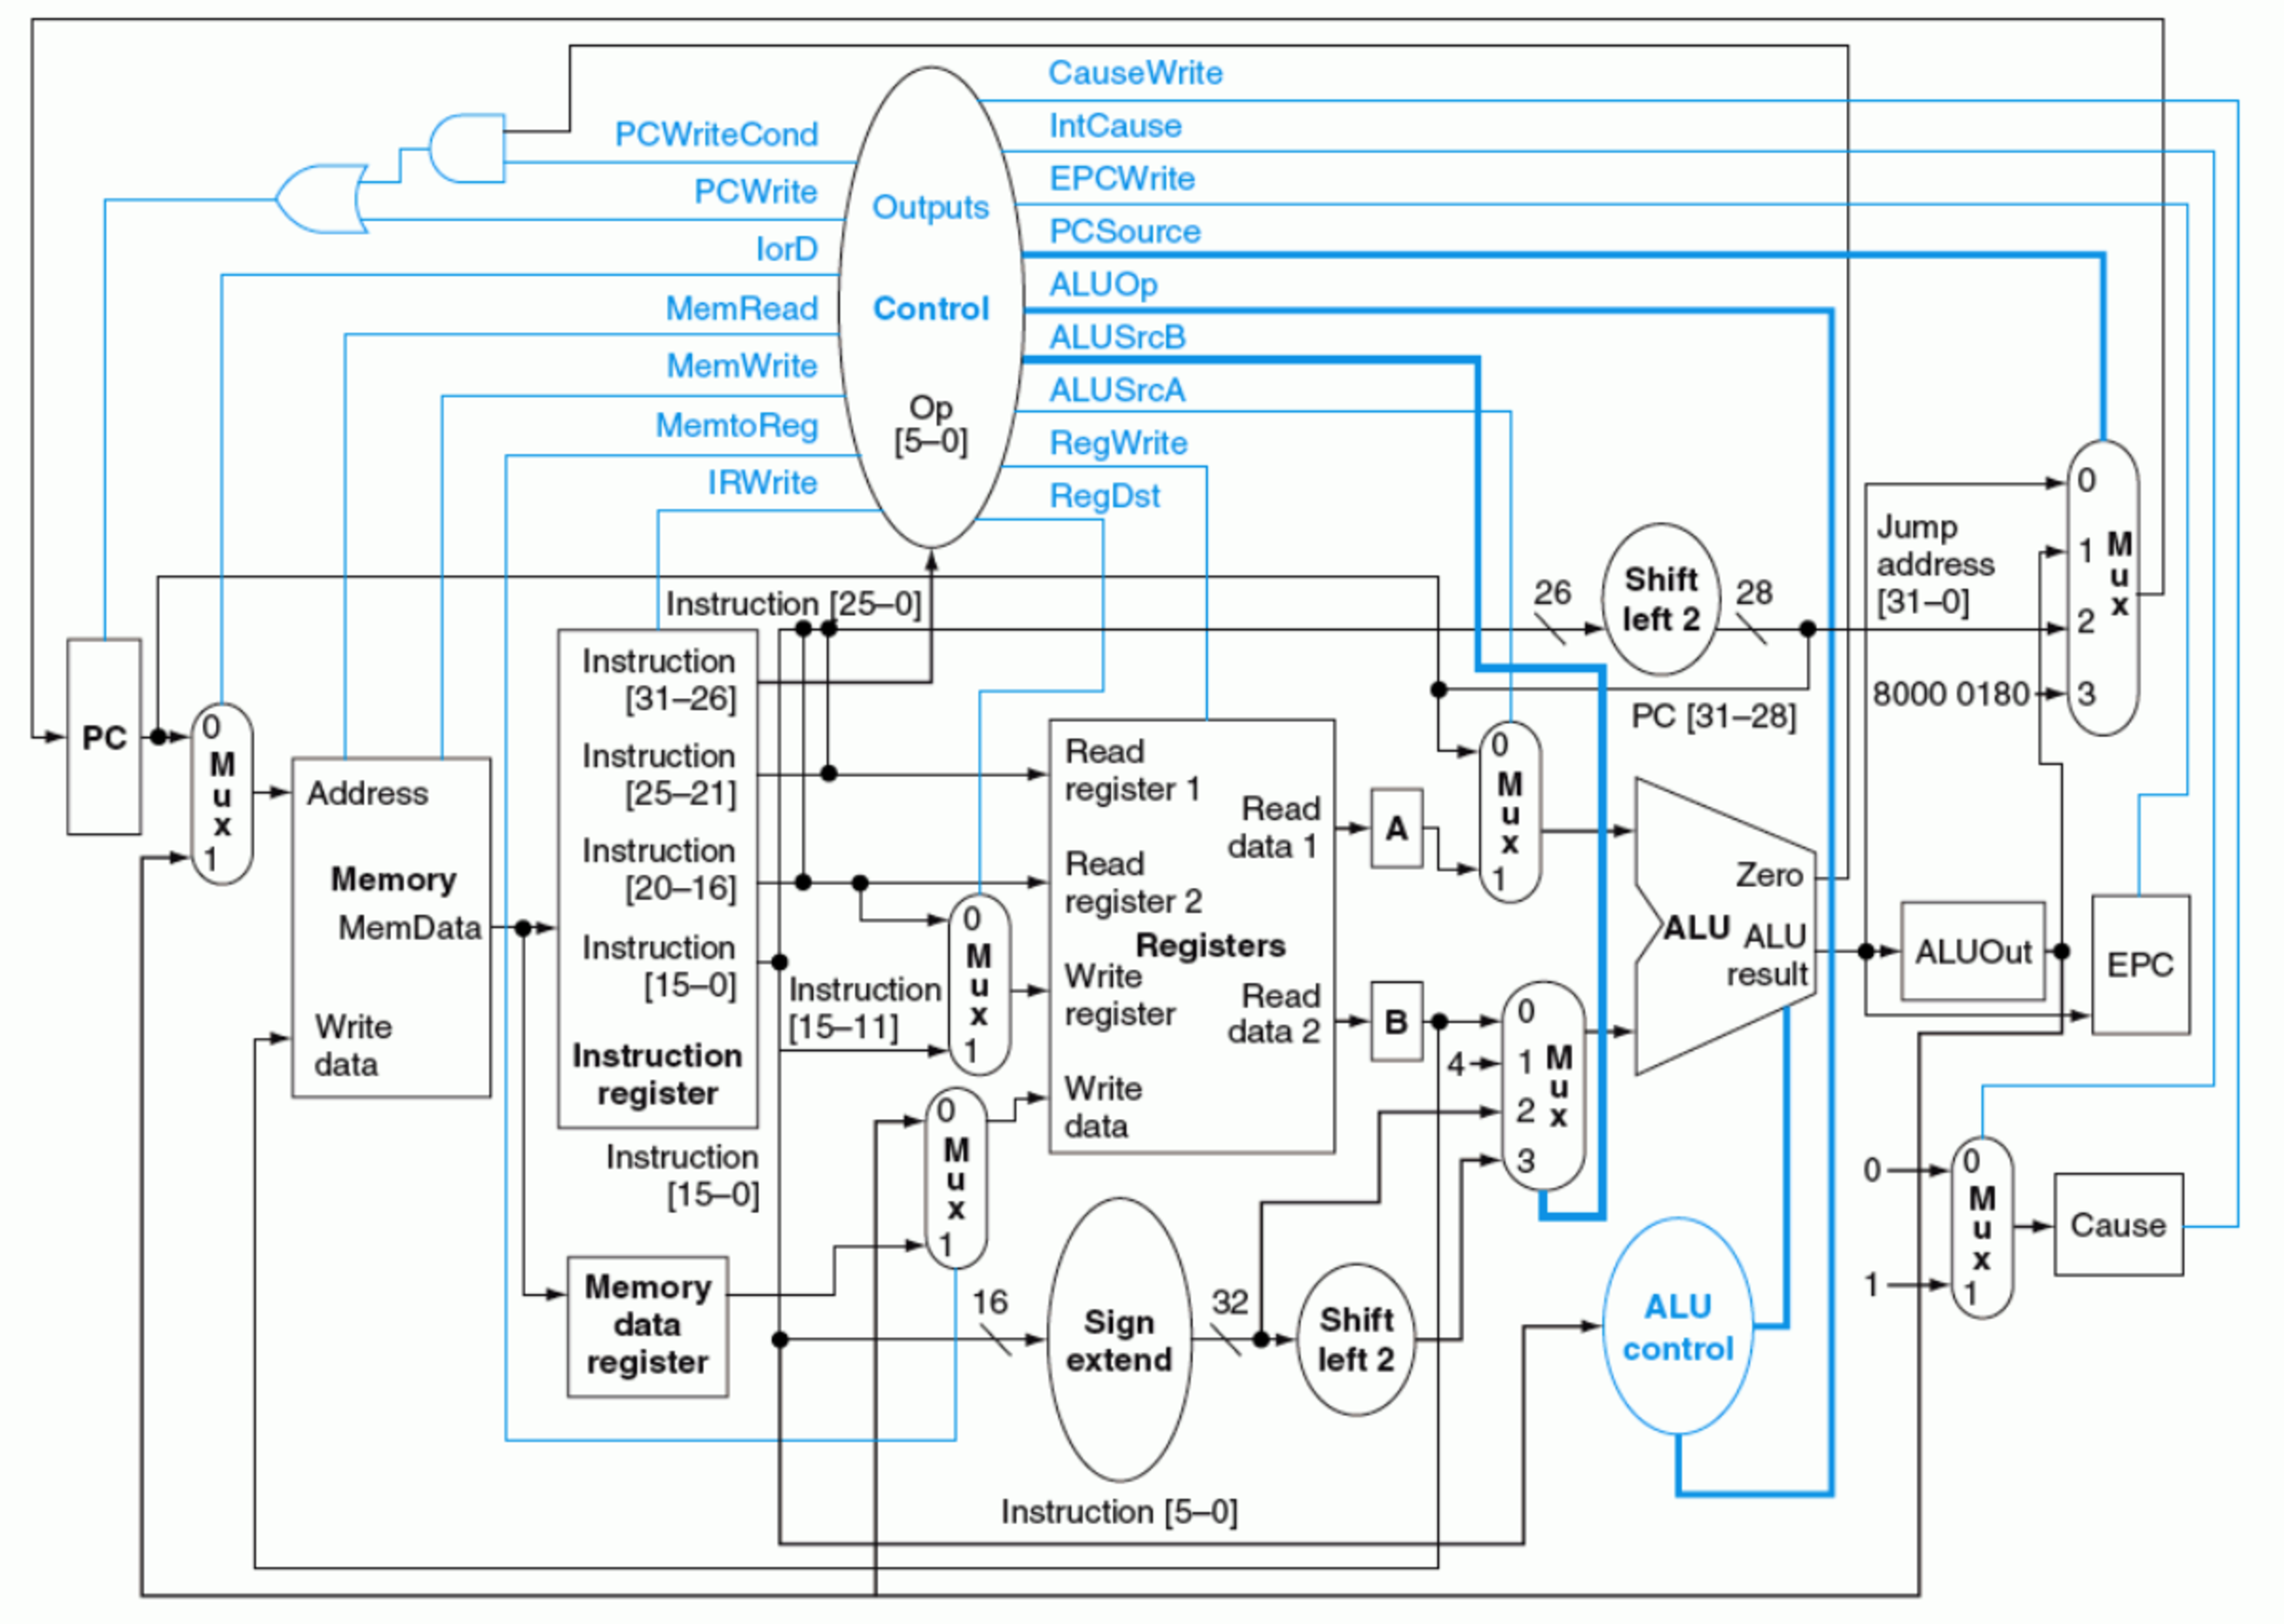
\includegraphics[width=6in]{./pics/multi-cycle-processor}
\caption{Microarchitecture for a multi-cycle {\it MIPS} processor \cite{Patterson2005}.}
\label{fig:multicycleprocessor}
\end{figure}



Figure \ref{fig:multicycleprocessorfsmctrllogic} shows the FSM for a multi-cycle {\it MIPS} processor \cite{Patterson2005,Patterson2005a}. It indicates the states that the processor can be in and how a state can transit to another state. The next state function determines the transition from the current state to the next state. The stages IF, ID, and WB are each represented as a stage in the FSM. Instructions that require the use of the ALU are categorized into memory access operations, execution, branch completion, and jump completion. Each category is represented as a state in the FSM. Similarly, the memory access operations for {\tt read} and {\tt write} are each represented as a state \cite{Patterson2005}. Subsection \ref{sssec:FiniteStateControl} briefly describes how this FSM can be mapped into a sequential circuit. \\

Figure \ref{fig:multicycleprocessor} shows the microarchitecture of the multi-cycle processor that includes the control path (colored in blue) and the datapath \cite{Patterson2005}. It integrates the datapath (see Figure \ref{fig:multicycleprocessordatapath2}) in Subsection \ref{ssec:DatapathDesignforMultiCycleProcessors} with the control logic (see Figure \ref{fig:controllogicmulticycleprocessor} in \S\ref{sssec:FiniteStateControl}) and associated wiring. It also has addition control logic for detecting and handling exceptions.








%%%%%%%%%%%%%%%%%%%%%%%%%%%%%%%%%%%%%%%%%%%
\subsubsection{Finite State Control}
\label{sssec:FiniteStateControl}

The process of implementing a FSM as a sequential circuit is described briefly as follows. \\

Firstly, label each state in the FSM as a binary number, which would be stored in a state register in the sequential circuit \cite{Patterson2005a}; a state register is a flip-flop circuit \cite{Kang2003a,Rabaey2003,Weste2011}. Next, represent each state and output signal in the FSM as a boolean variable. Determine a boolean function of states to obtain the boolean value for each output signal in the FSM. The combinational circuit derived from this boolean function is the output logic circuit for the FSM. Subsequently, design the combinational circuit needed to determine the next state for a given state in the FSM. That is, for each possible next state in the FSM, represent that state as a boolean variable. The value of the boolean variable is determined by a boolean function of the states and output signals of the FSM. Here, each state or output signal is represented as a boolean variable. The second boolean function is mapped to a combinational circuit. This combinational circuit is called the next state logic circuit for the FSM. \\


\begin{figure}[h]
\centering 
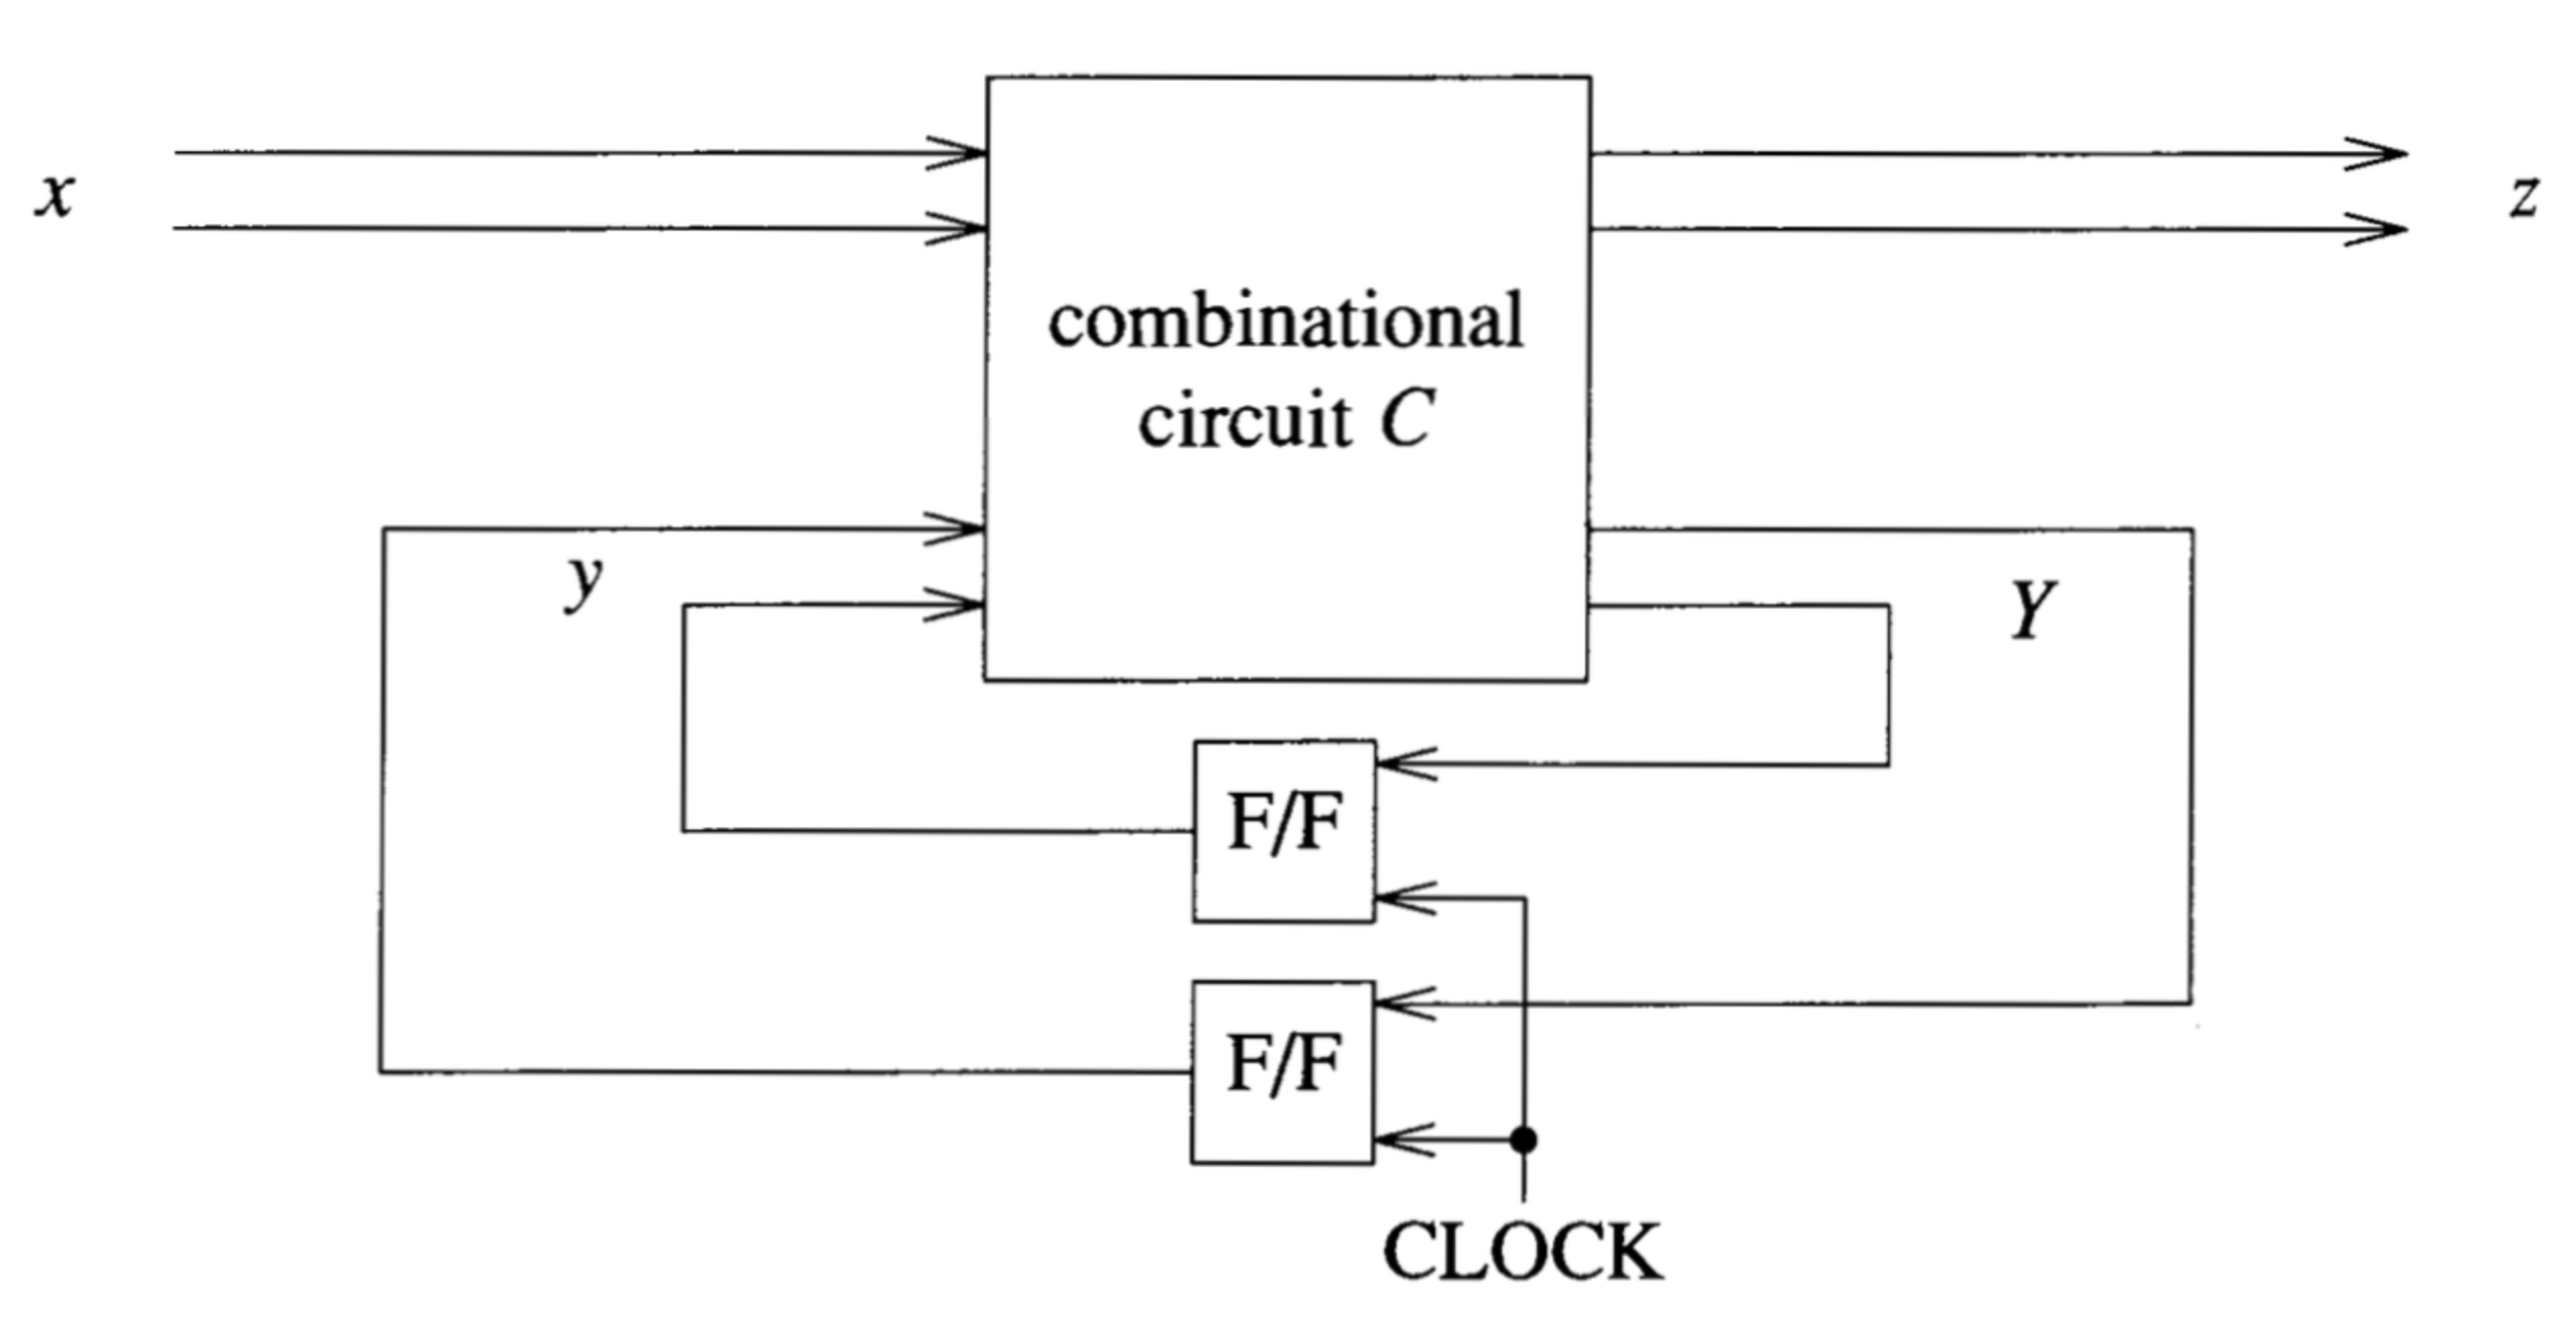
\includegraphics[width=4in]{./pics/canonical-sequential-logic-circuit}
\caption{A schematic for the canonical circuit topology for a synchronous sequential circuit. The clock signal {\tt CLOCK} provides synchrony for the sequential circuit. The combinational circuit {\it C} represents the next state logic and output logic circuits of the sequential circuit's finite state machine (FSM) representation, and the pair of flip-flops (F/F) provide the state storage for the FSM \cite{Abramovici1990}.}
\label{fig:canonicalsequentiallogiccircuit}
\end{figure}
%	Figure 2.5, pp. 14, \cite{Abramovici1990}

Figure \ref{fig:canonicalsequentiallogiccircuit} shows the canonical circuit topology for a synchronous sequential circuit, which encapsulates the next state logic and the output logic circuits as the combinational circuit {\it C} and represents state storage as a pair of flip-flops (F/F). The clock signal {\tt CLOCK} indicates that this sequential circuit is synchronous. Figure \ref{fig:controllogicmulticycleprocessor} shows a schematic for a sequential circuit implementing the FSM (see Figure \ref{fig:multicycleprocessorfsmctrllogic}) of the multi-cycle {\it MIPS} processor's control unit in this canonical structure. \\

\begin{figure}[h]
\centering 
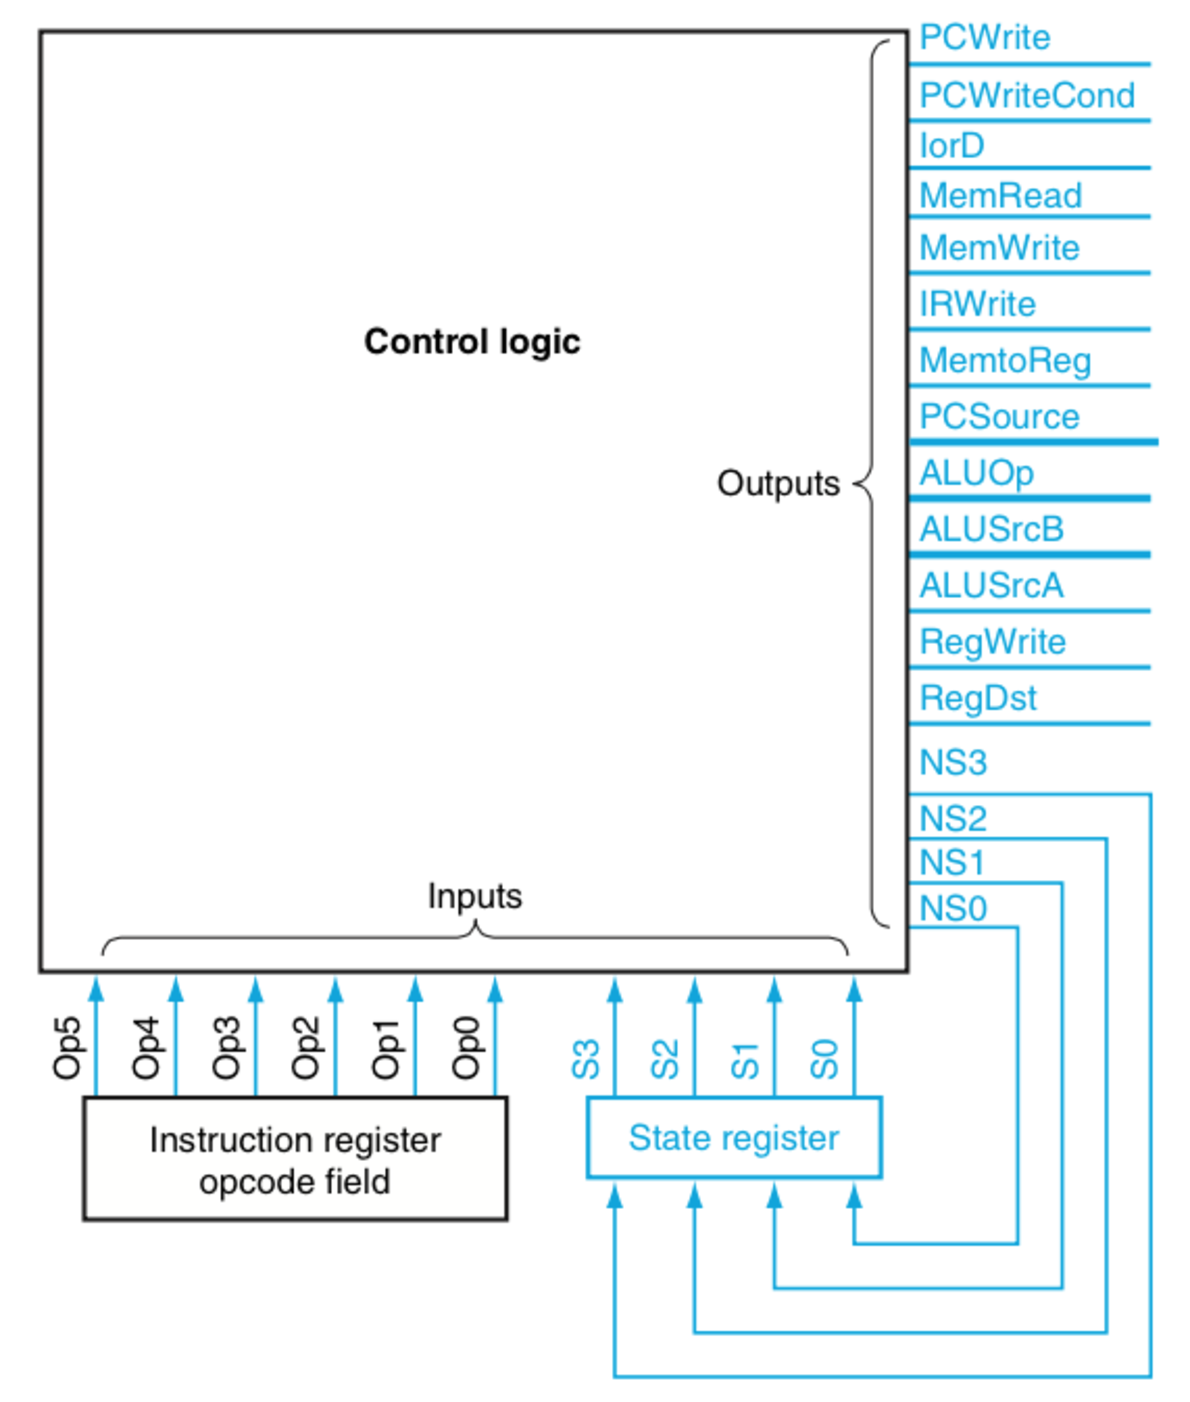
\includegraphics[width=4in]{./pics/control-logic-multi-cycle-processor}
\caption{A sequential circuit representing the FSM for the control unit of the multi-cycle {\it MIPS} processor \cite{Patterson2005a}. Its circuit topology has the canonical structure of sequential circuits shown in Figure \ref{fig:canonicalsequentiallogiccircuit}. The state register provide the state storage, and the control logic includes the next state logic and the output logic circuits needed to implement the FSM for the control unit of the processor.}
\label{fig:controllogicmulticycleprocessor}
\end{figure}
%	Figure D.3.2, pp. D-10, \cite{Patterson2005a}

The combinational circuit {\it C} in Figure \ref{fig:canonicalsequentiallogiccircuit} or the control logic in Figure \ref{fig:controllogicmulticycleprocessor} can be implemented using standard cells\cite{Kang2003a,Rabaey2003,Weste2011}, a read-only memory (ROM) device, or a programmable logic array (PLA). The ROM device or PLA encodes the truth tables for the boolean functions in the combinational circuit {\it C}.

%%%%%%%%%%%%%%%%%%%%%%%%%%%%%%%%%%%%%%%%%%%
\subsection{Advantages and Disadvantages of Multi-Cycle Processor Design}
\label{ssec:AdvantagesandDisadvantagesofMultiCycleProcessorDesign}

The advantage of the multi-cycle processor design over the microarchitecture for the single-cycle microarchitecture is the lower amount of hardware resources that are required in the datapath. From Equation \ref{eqn:ironlaw}, we can relatively compare the performance of the multi-cycle processor with the single-cycle processor. The CPI for the multi-cycle processor is higher than that of the single-cycle processor, since the multi-cycle processor takes multiple cycles to complete executing each instruction. However, the multi-cycle processor has a lower clock cycle period. If the normalized decrease in the clock period of the multi-cycle processor is relatively greater than the normalized increase in the CPI of the multi-cycle processor, the multi-cycle processor would have better performance than the single-cycle processor.




%%%%%%%%%%%%%%%%%%%%%%%%%%%%%%%%%%%%%%%%%%%
\subsection{Microprogramming}
\label{ssec:Microprogramming}

%In contemporary processors, there are ISAs that include more than 100 instructions, and these instructions can have clock cycle latencies ranging from 1 to 20 CPI. Therefore, manually detailing the control signals in a schematic of the VLSI circuit implementation of a microarchitecture is error prone. Likewise, a FSM representation of the control unit of a processor would be cumbersome to manually describe, too. There would be too many states (i.e., more than 1000 states) in the FSM representation. This means that it would be very difficult to verify such large FSMs \cite{Patterson2005a}. \\

Contemporary processors implement ISAs that include more than 100 instructions, and these instructions can have clock cycle latencies ranging from 1 to 20 CPI. Therefore, manually detailing the control signals in a schematic of the VLSI circuit implementation of a microarchitecture is error prone. Likewise, a FSM representation of the control unit of a processor would be cumbersome to manually describe too. There would be too many states (i.e., more than 1000 states) in the FSM representation. This means that it would be very difficult to verify such large FSMs \cite{Patterson2005a}. \\

Therefore, microprogramming is used to address this processor design challenge by treating each set of control signals as a microinstruction (or low-level control instruction) that can be executed by the datapath. This instruction would represent a state in the FSM for the control unit. That is, for each state in the FSM of the control unit, represent the output control signals from that state as a microinstruction to be executed in the datapath. It allows a set of (datapath) control signals to be symbolically represented as a microprogram, which consists of multiple microinstructions. Since many instructions in an ISA, such as the {\it MIPS} ISA, would share common sequences of microinstructions, a lot of code reuse of these common sequences (or microcode) occurs. Representing control signals as microcode/microprograms instead of wires, buses, and digital circuits allow the design of a microarchitecture to have a simpler control path \cite{Patterson2005a}. \\



















